\section{実データ解析}
本節では実データを解析する.

\subsection{実データ}
本研究で用いるデータは筑波大学の柳沢研究所で計測されたカルシウムイメージングデータである.
本データは,2光子多細胞カルシウムイメージングによって1匹のマウスの大脳皮質1次運動野第2・3層のニューロンのイメージング画像を得た後,人手でROIがつけられ,ニューロンごとの数値データに直されたものである.
通常の睡眠状態と睡眠を阻害した状態の計測が別日に行われた.
ただし,観測ニューロンは同じである.
1時間おきに15分間のイメージングがそれぞれ6回と5回行われた.
イメージングのサンプリングレートは8[Hz]である.
用いられた蛍光タンパク質はGCaMP6sである.
実験系は\Figref{fig:imaging}(A)の系で行われた\cite{Kanda2016}.
観測されたニューロン数は154であった.
時間方向には4[s]ごとのマウスの状態(wake, REM, NREM)のラベルが付いており,ニューロンごとに興奮性か抑制性のラベルがついている.
通常睡眠データと阻害睡眠データの時系列方向のラベルをそれぞれ\Figref{fig:normal-state}と\Figref{fig:deprivation-state}に示す.

\begin{figure}[htbp]
    \begin{center}
				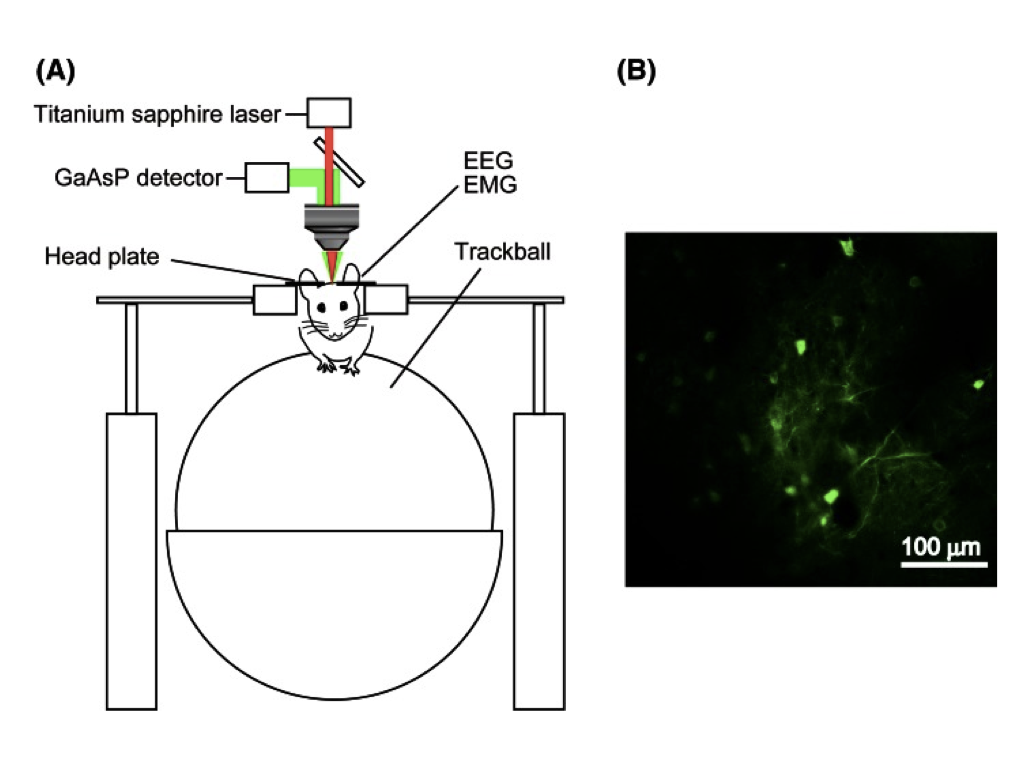
\includegraphics[width=0.8\linewidth]{imaging}
				\caption{(A)カルシウムイメージングの測定系.マウスは頭を固定されたままボールの上で活動することができる.(B)カルシウムイメージング画像.}
        \label{fig:imaging}
    \end{center}
\end{figure}

\begin{figure}[htbp]
	\begin{minipage}{0.5\hsize}
		\begin{center}
			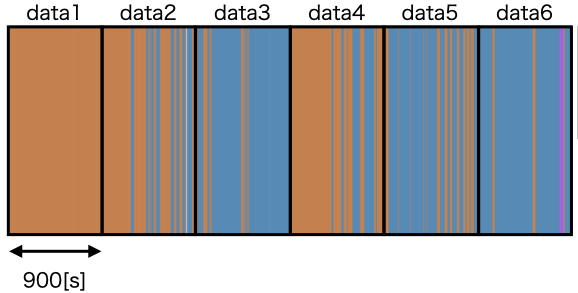
\includegraphics[width=\hsize]{normal-state}
			\caption{通常睡眠データのラベル}
			\label{fig:normal-state}
		\end{center}
	\end{minipage}
	\begin{minipage}{0.5\hsize}
		\begin{center}
				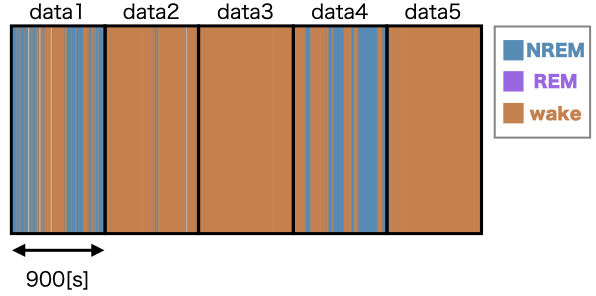
\includegraphics[width=\hsize]{deprivation-state}
				\caption{阻害睡眠データのラベル}
				\label{fig:deprivation-state}
		\end{center}
	\end{minipage}
\end{figure}

\subsection{提案アプローチのクラスタリング結果}
15分のデータごとに提案アプローチを用いてクラスタリングを行う.
NMFを一回行い,それを最尤推定の結果とする.
最尤推定結果からBICを計算し,目視で基底数4つを決める.
NMFの設定を\Tabref{tab:exp4param2}に示す.
$\bar{A}$の閾値を0.5としてグループに所属しないニューロンを除外する.
クラスタ数は人工データ実験の時と同様に固有値ギャップからプログラムを使って求めるが,あまりに大きすぎるクラスタ数の場合(例えば152など)は目視で決定した.

\begin{table}[htb]
  \center
  \begin{tabular}{c|c} \hline
		1回の結果を出すNMFの回数 & 100 \\
		基底数 & BIC最大周りの4つの数 \\
		ブートストラップサンプル数 & 100 \\
		ブートストラップ方法 & 残差型ブートストラップ \\ \hline
  \end{tabular}
  \caption{NMFの設定}
  \label{tab:exp4param2}
\end{table}

% 推定された通常睡眠データのクラスタを\Figref{fig:real-clstn}に,阻害睡眠データのクラスタを\Figref{fig:real-clstd}に示す.
% ニューロンは実際の座標に丸として示され,同じクラスタのニューロンは同じ色となっている.
% グループに所属しないニューロンは黒丸となっている.
% 
% \begin{figure}[htbp]
%     \begin{minipage}{0.32\hsize}
% 			\begin{center}
% 					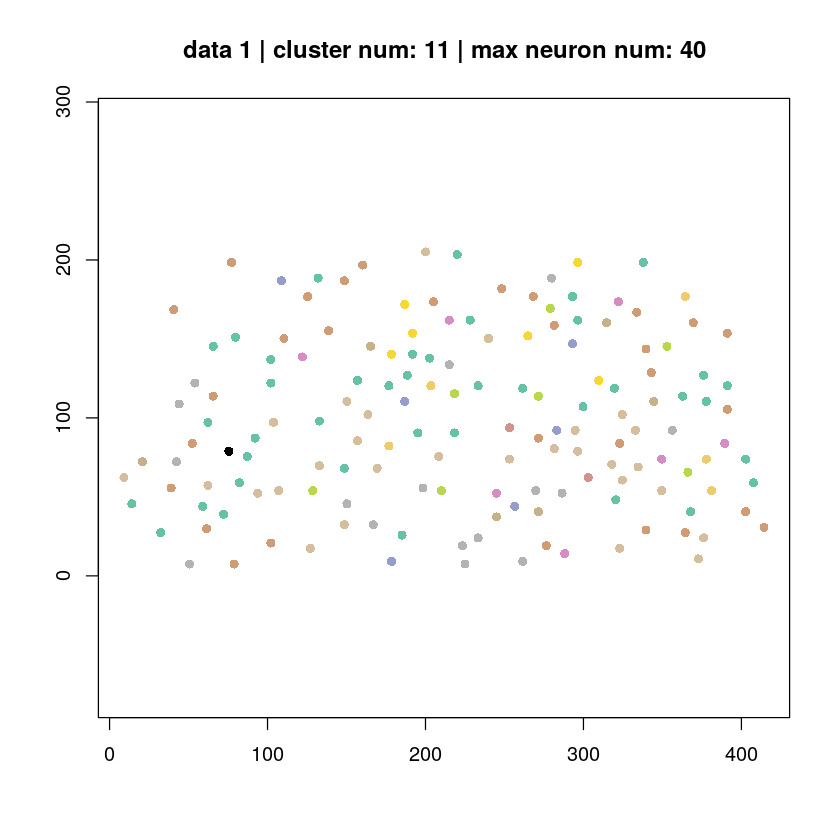
\includegraphics[width=\hsize]{clustern1} \end{center}
% 		\end{minipage}
%     \begin{minipage}{0.32\hsize}
% 			\begin{center}
% 					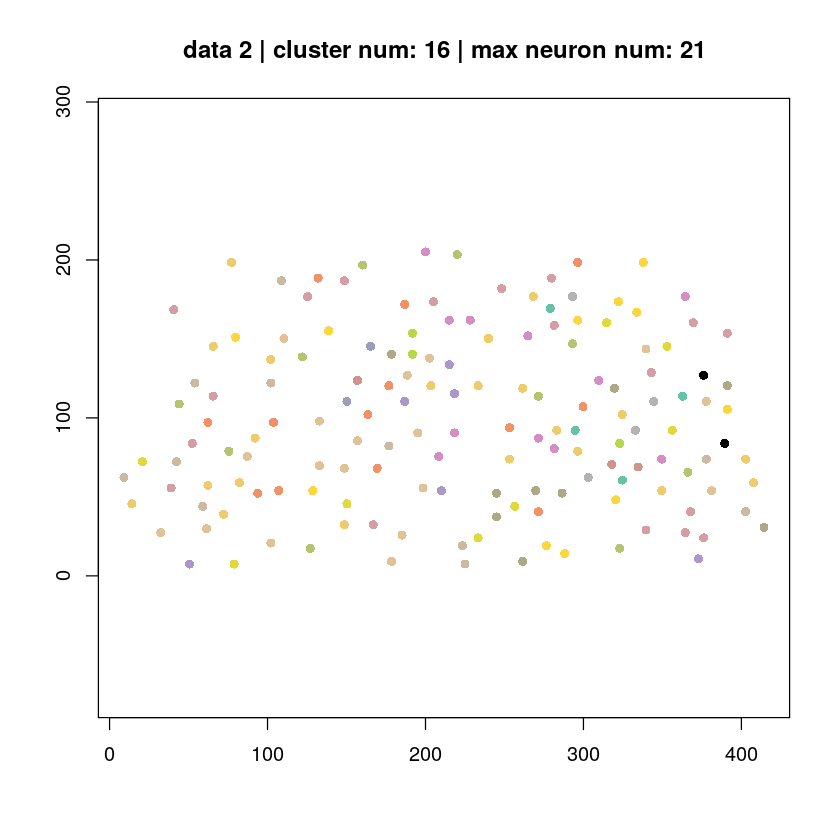
\includegraphics[width=\hsize]{clustern2}
% 			\end{center}
% 		\end{minipage}
%     \begin{minipage}{0.32\hsize}
% 			\begin{center}
% 					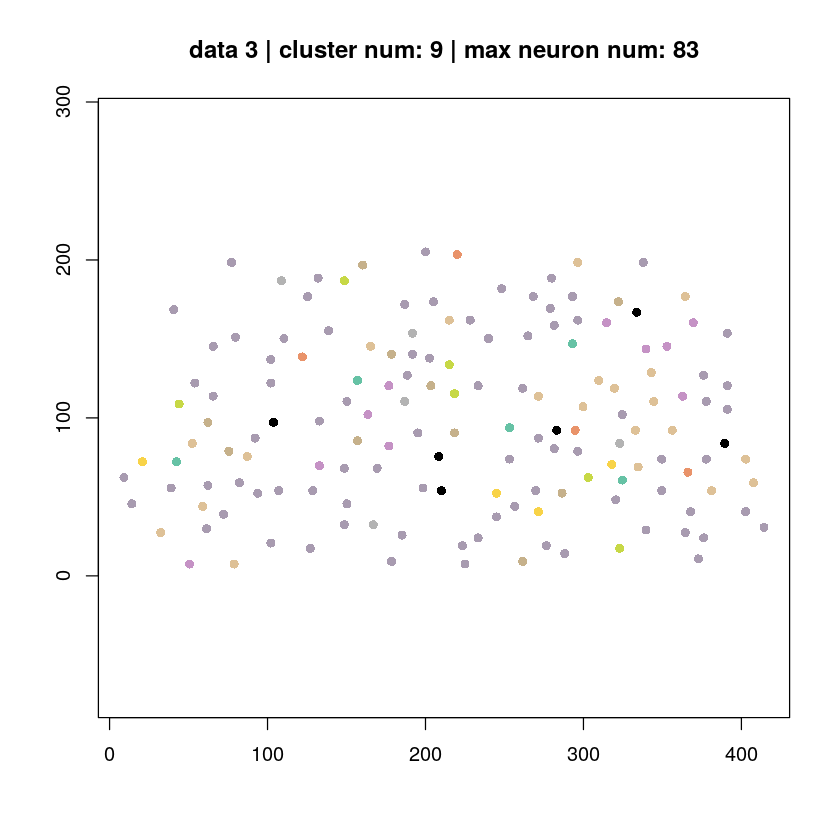
\includegraphics[width=\hsize]{clustern3}
% 			\end{center}
% 		\end{minipage}\\
%     \begin{minipage}{0.32\hsize}
% 			\begin{center}
% 					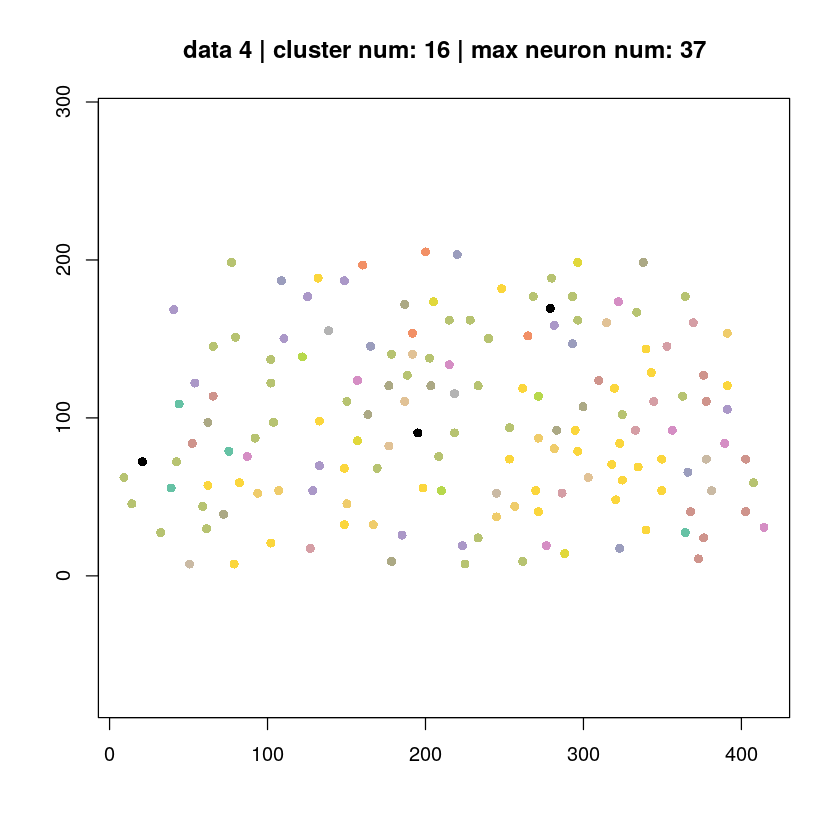
\includegraphics[width=\hsize]{clustern4}
% 			\end{center}
% 		\end{minipage}
%     \begin{minipage}{0.32\hsize}
% 			\begin{center}
% 					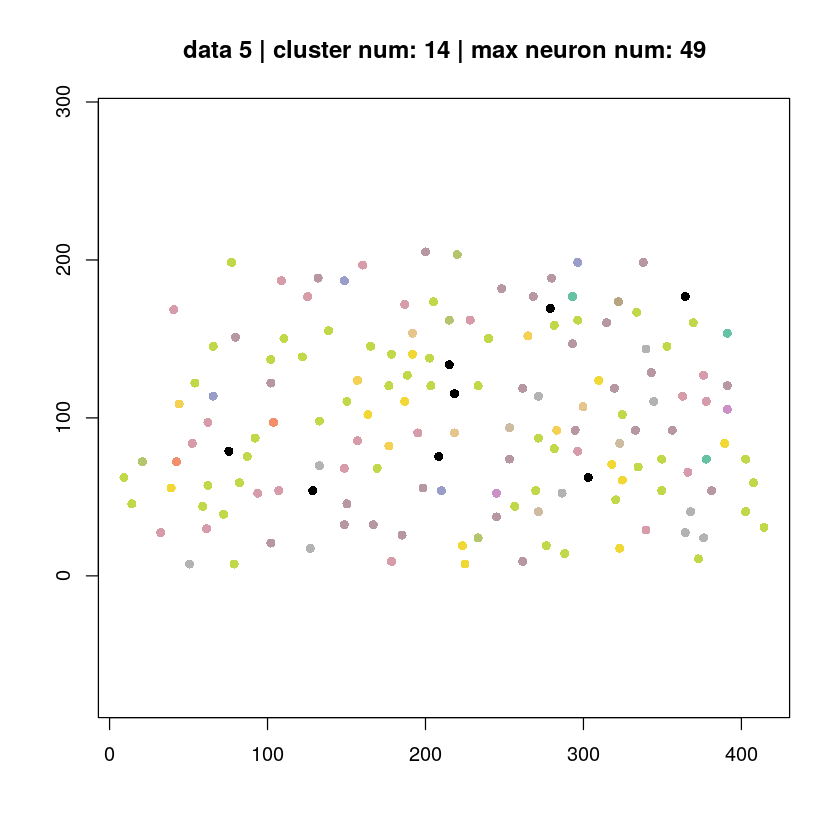
\includegraphics[width=\hsize]{clustern5}
% 			\end{center}
% 		\end{minipage}
%     \begin{minipage}{0.32\hsize}
% 			\begin{center}
% 					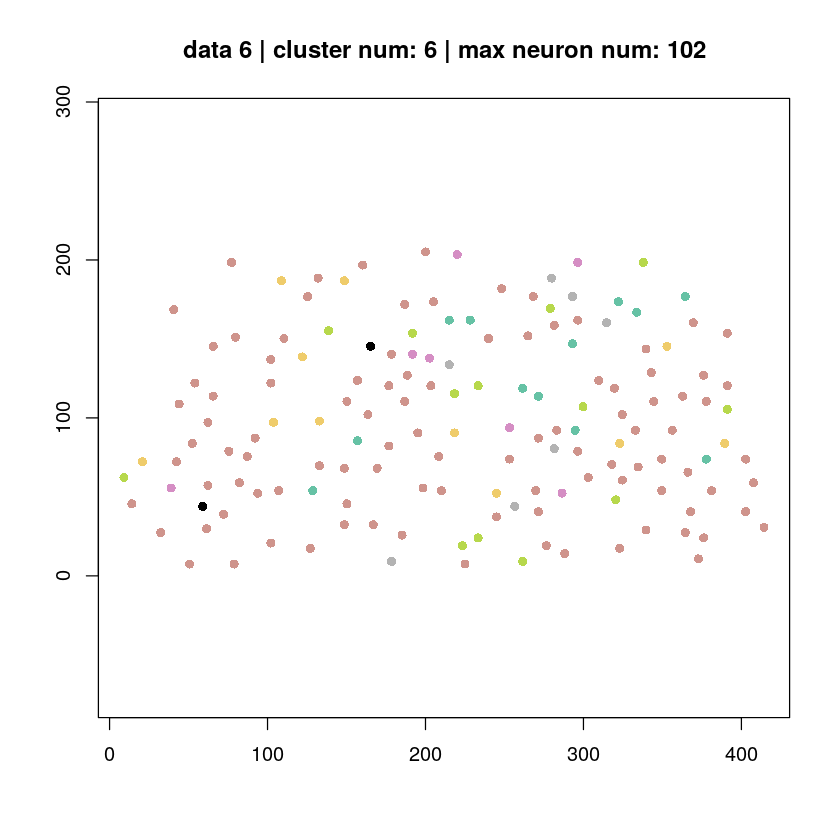
\includegraphics[width=\hsize]{clustern6}
% 			\end{center}
% 		\end{minipage}
% 		\label{fig:real-clstn}
% \end{figure}
% 
% \begin{figure}[htbp]
%     \begin{minipage}{0.32\hsize}
% 			\begin{center}
% 					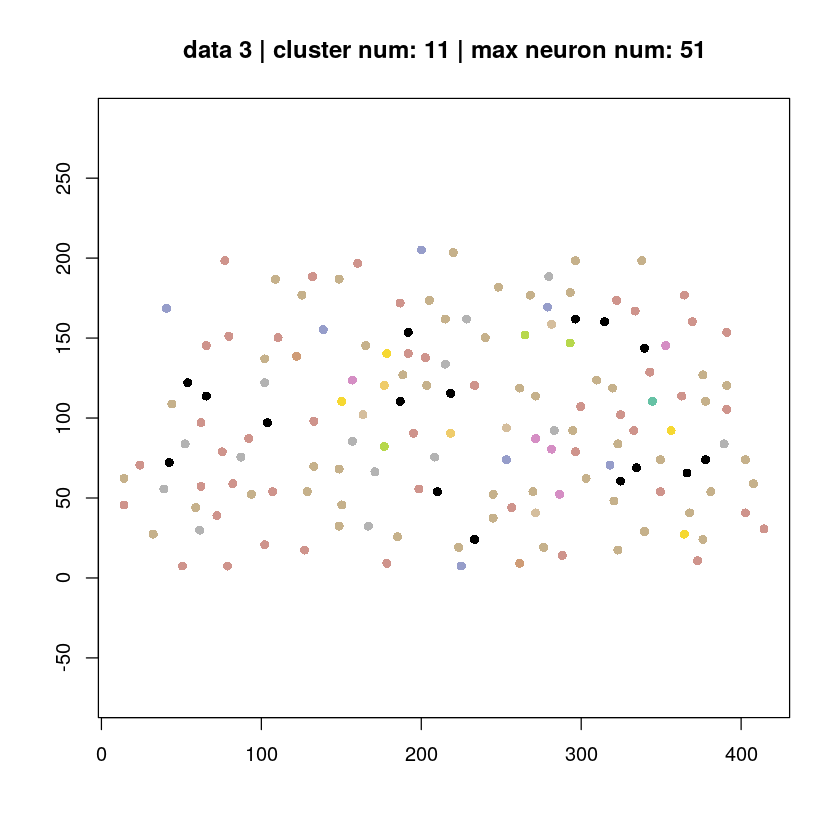
\includegraphics[width=\hsize]{clusterd3}
% 			\end{center}
% 		\end{minipage}
%     \begin{minipage}{0.32\hsize}
% 			\begin{center}
% 					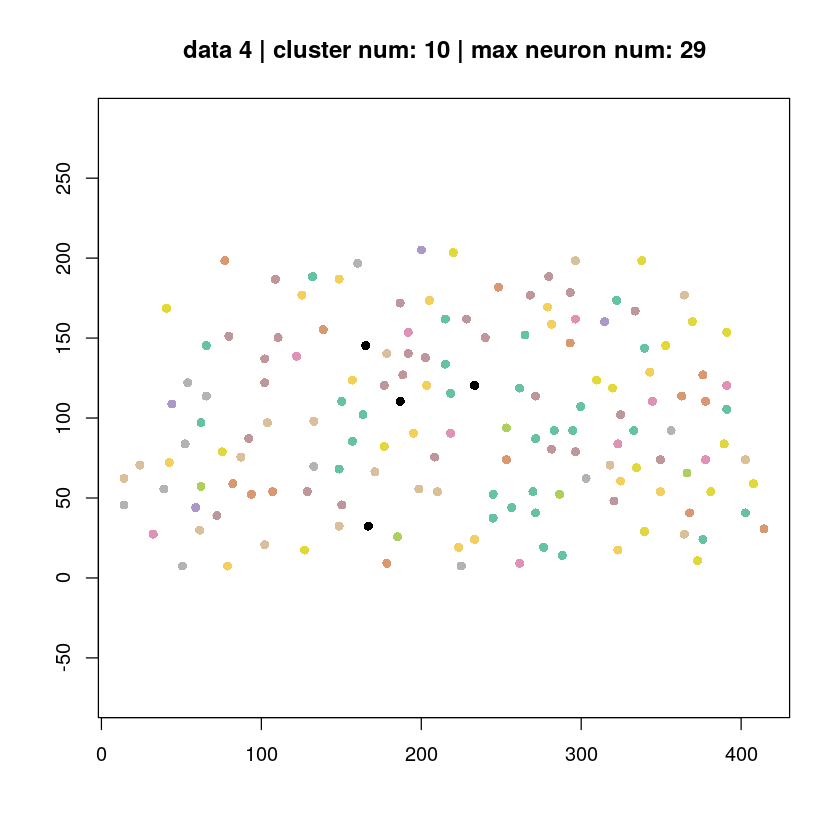
\includegraphics[width=\hsize]{clusterd4}
% 			\end{center}
% 		\end{minipage}
%     \begin{minipage}{0.32\hsize}
% 			\begin{center}
% 					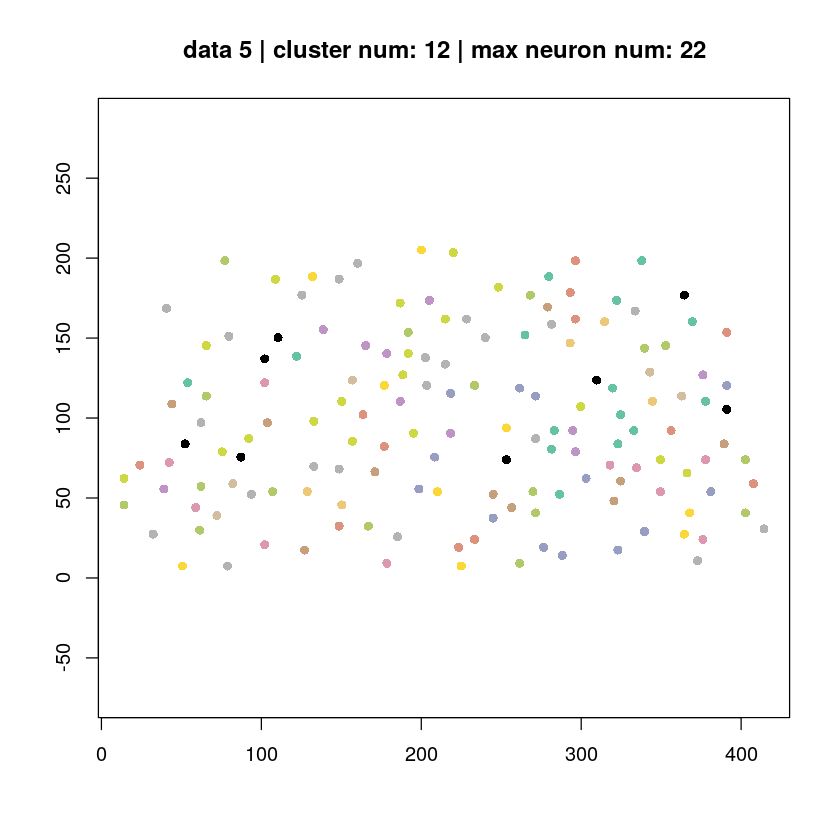
\includegraphics[width=\hsize]{clusterd5}
% 			\end{center}
% 		\end{minipage}\\
%     \begin{minipage}{0.32\hsize}
% 			\begin{center}
% 					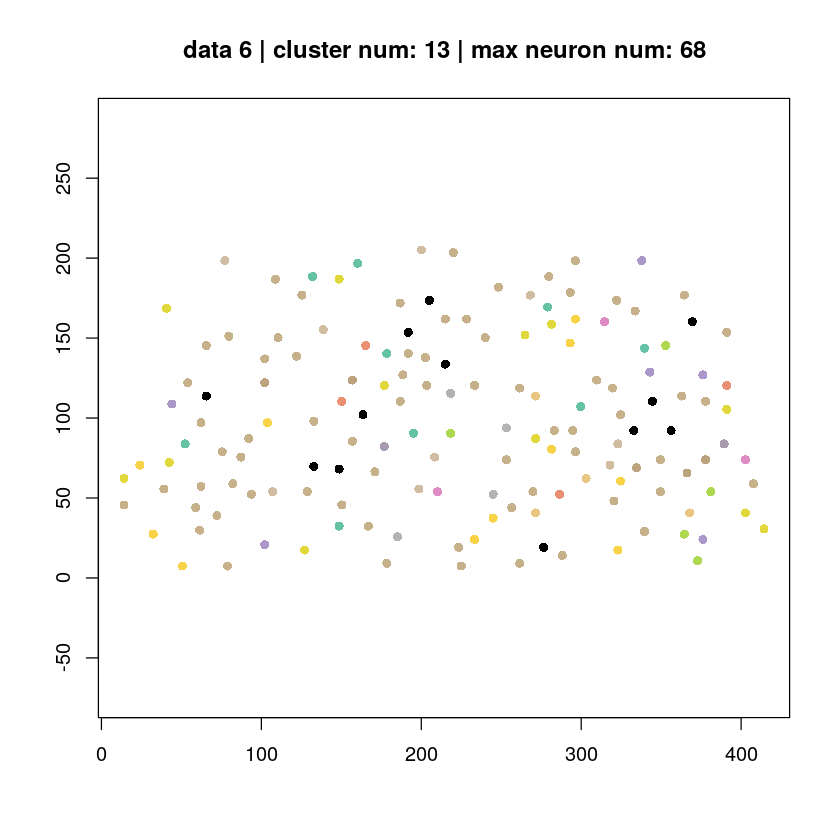
\includegraphics[width=\hsize]{clusterd6}
% 			\end{center}
% 		\end{minipage}
%     \begin{minipage}{0.32\hsize}
% 			\begin{center}
% 					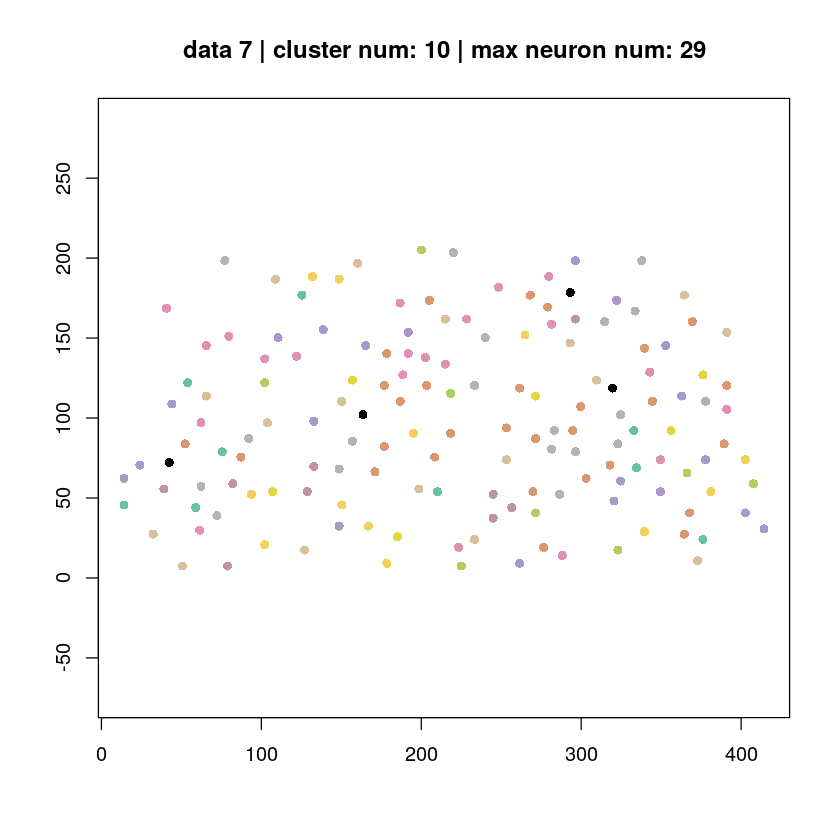
\includegraphics[width=\hsize]{clusterd7}
% 			\end{center}
% 		\end{minipage}
% 		\label{fig:real-clstd}
% \end{figure}

推定された通常睡眠データのクラスタ内ニューロン数を\Figref{fig:normal-clstnums}に,阻害睡眠データのクラスタ内ニューロン数を\Figref{fig:normal-clstnums}に示す.
\Figref{fig:normal-state}と\Figref{fig:deprivation-state}と見比べると,睡眠時に大規模クラスタが存在していることがわかる.

\begin{figure}[htbp]
	\begin{minipage}{0.5\hsize}
		\begin{center}
			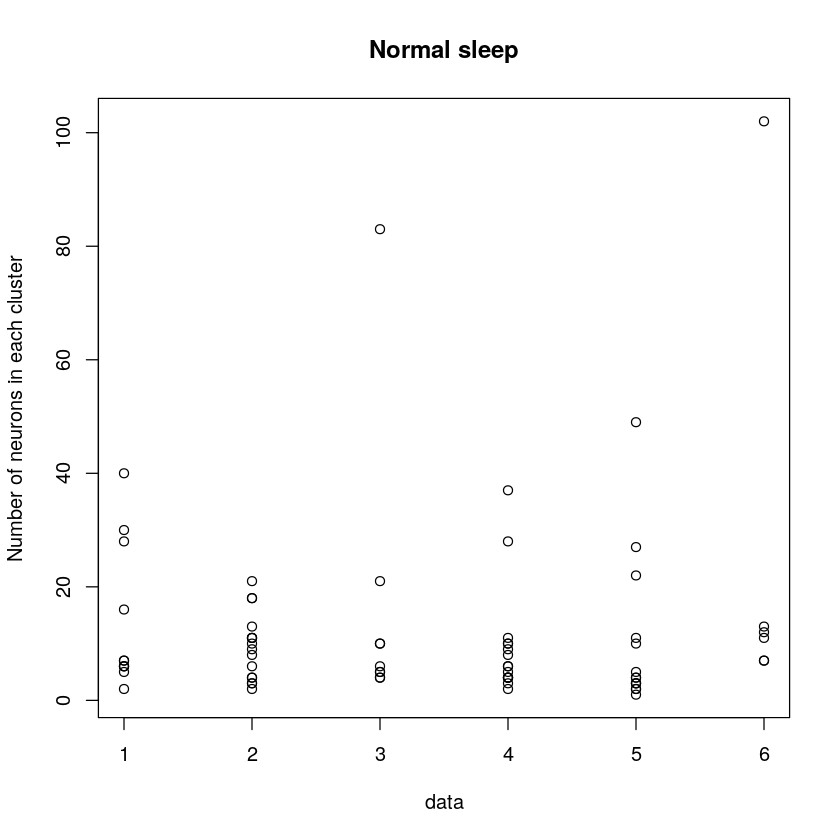
\includegraphics[width=\hsize]{normal-clstnums}
			\caption{通常睡眠データから推定されたクラスタに含まれるニューロン数.}
			\label{fig:normal-clstnums}
		\end{center}
	\end{minipage}
	\begin{minipage}{0.5\hsize}
		\begin{center}
				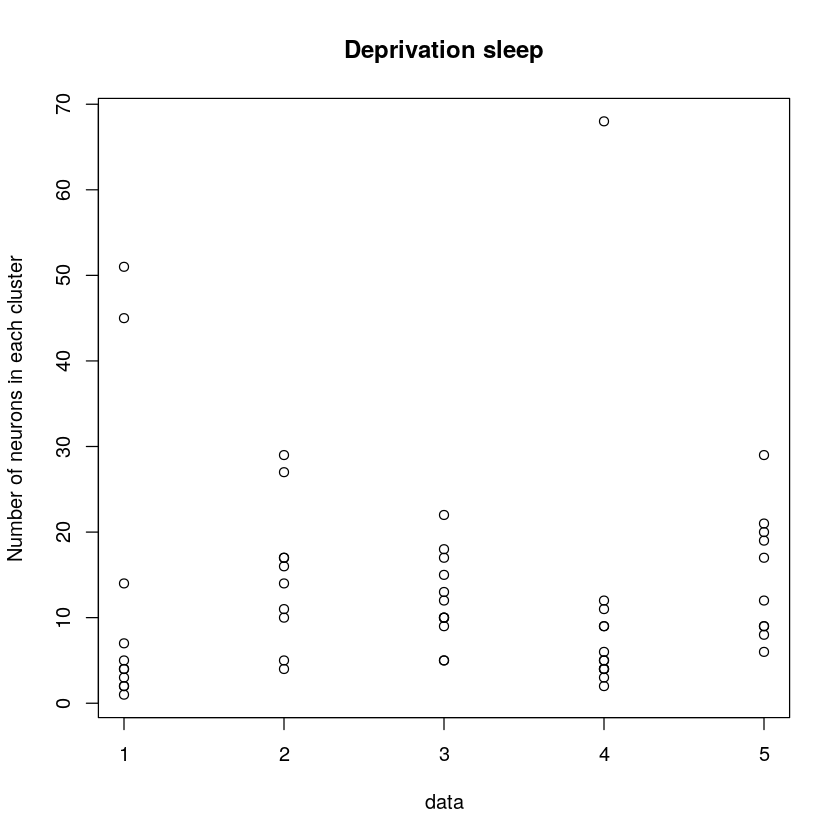
\includegraphics[width=\hsize]{deprivation-clstnums}
				\caption{阻害睡眠データから推定されたクラスタに含まれるニューロン数.}
				\label{fig:deprivation-clstnums}
		\end{center}
	\end{minipage}
\end{figure}

推定されたクラスタにデータ間で被りがあるかを見るため,各データペアでクラスタ間のJaccard係数を計算した.
通常睡眠データ内で比較した結果を\Figref{fig:nn-jaccard}に示す.
例えばデータ1で11個のクラスタが推定され,データ2で16個のクラスタが推定されたが,\Figref{fig:normal-clstnums}の``n1-n2"はデータ1の各クラスタとデータ2の各クラスタのJaccard係数を計算し,データ1のクラスタそれぞれで最大となった係数をプロットしている.
同様に,阻害睡眠データ内で比較した結果を\Figref{fig:dd-jaccard}に,通常睡眠データと阻害睡眠データで比較した結果を\Figref{fig:dn-jaccard}に示す.
この結果から,``n3-n6",``n6-n3",``n3-d4",``n6-d4"でJaccard係数が大きくなっていることがわかる.
これらのクラスタは,\Figref{fig:normal-clstnums}と\Figref{fig:deprivation-clstnums}のクラスタ内ニューロン数が多いクラスタであった.
また,この3つのデータ(通常睡眠のデータ3とデータ6,阻害睡眠のデータ4)はNREM睡眠が半分ほどを占めているデータである.
これより,この3つのクラスタ全てに所属するニューロンがNREM睡眠中に同時活動している可能性がある.
他にもJaccard係数が0.4近いクラスタペアもあるが,クラスタ内ニューロン数が少なかったため今回は議論しない.

\begin{figure}[htbp]
    \begin{center}
				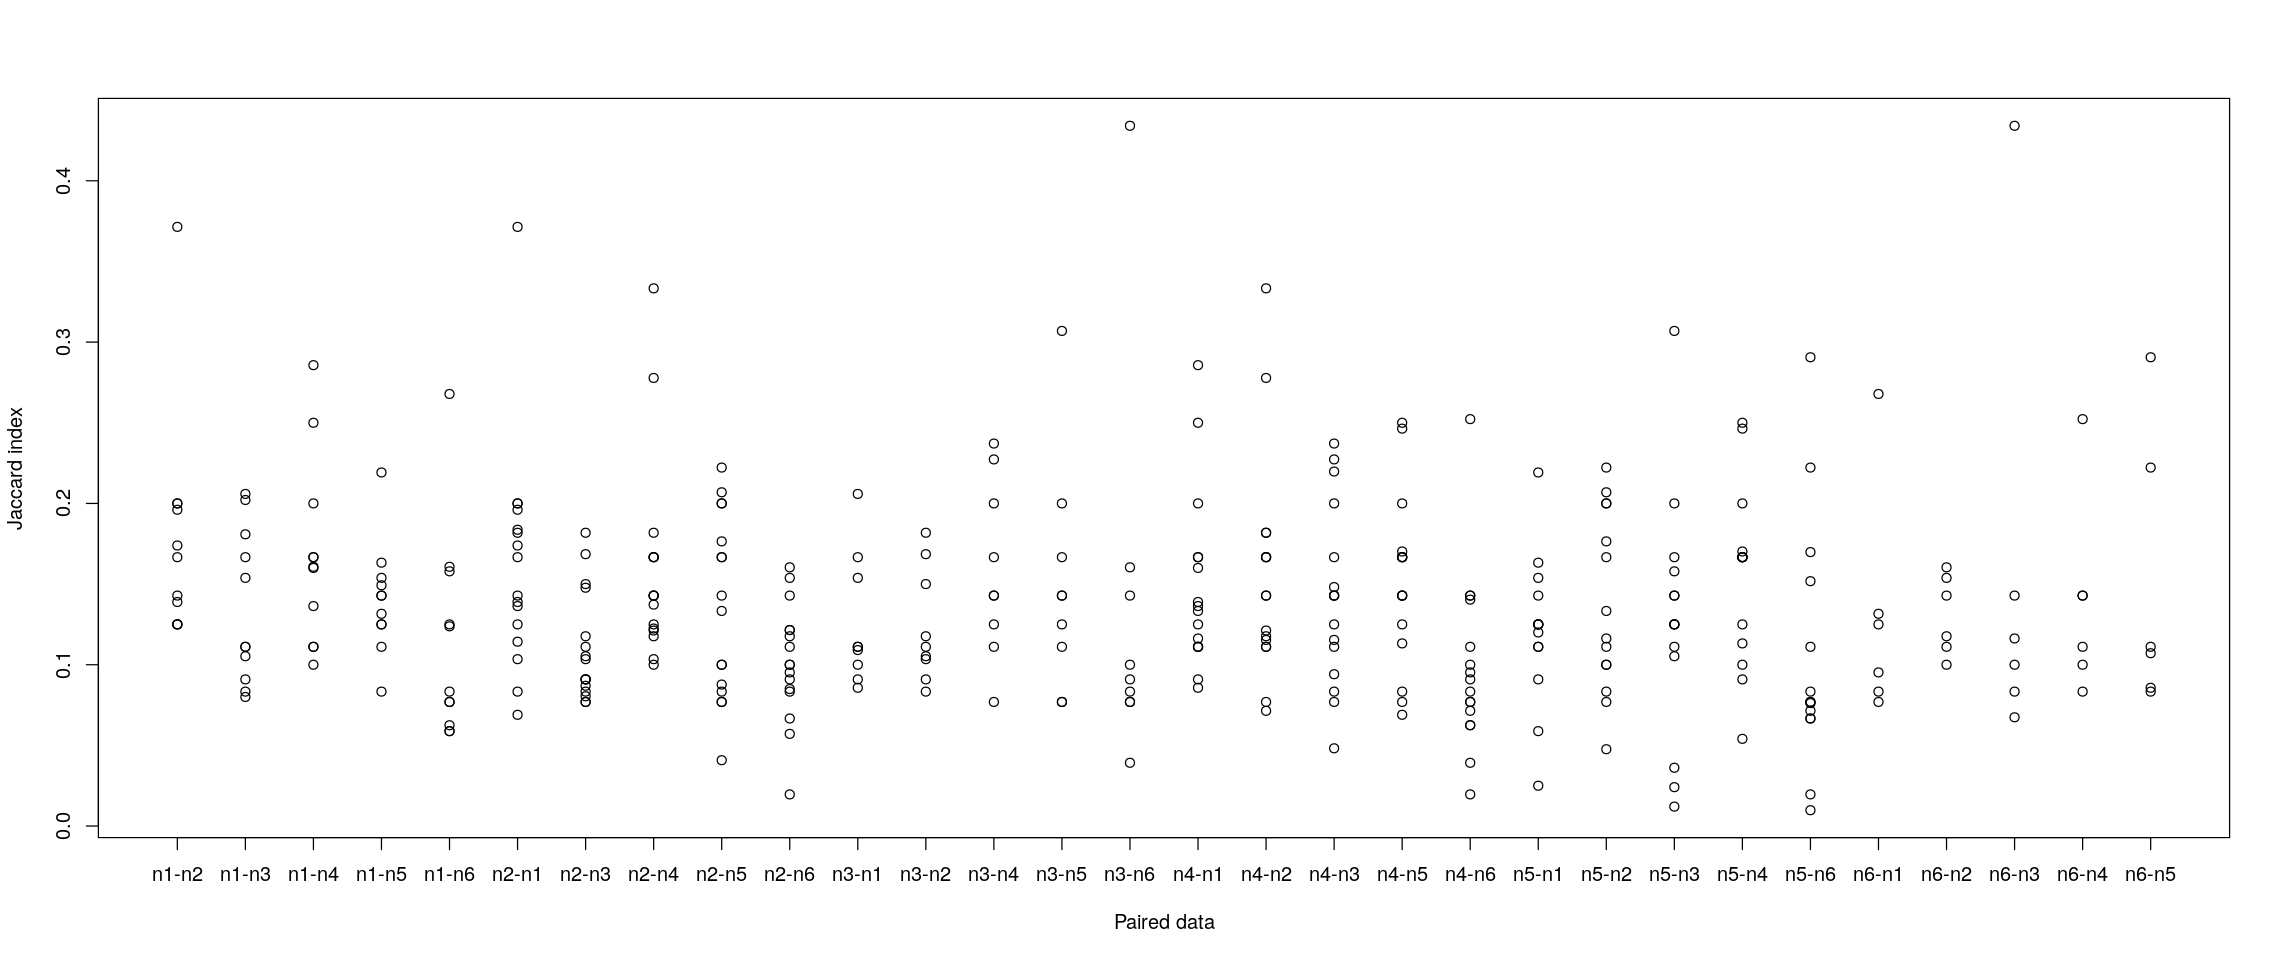
\includegraphics[width=\linewidth]{nn-jaccard}
				\caption{通常睡眠データペアで各クラスタのJaccard係数を計算した図.横軸のラベルはデータペアを表し,``n1-n2"はデータ1とデータ2のクラスタ間でJaccard係数を計算した.}
        \label{fig:nn-jaccard} \end{center}
\end{figure}
\begin{figure}[htbp]
    \begin{center}
				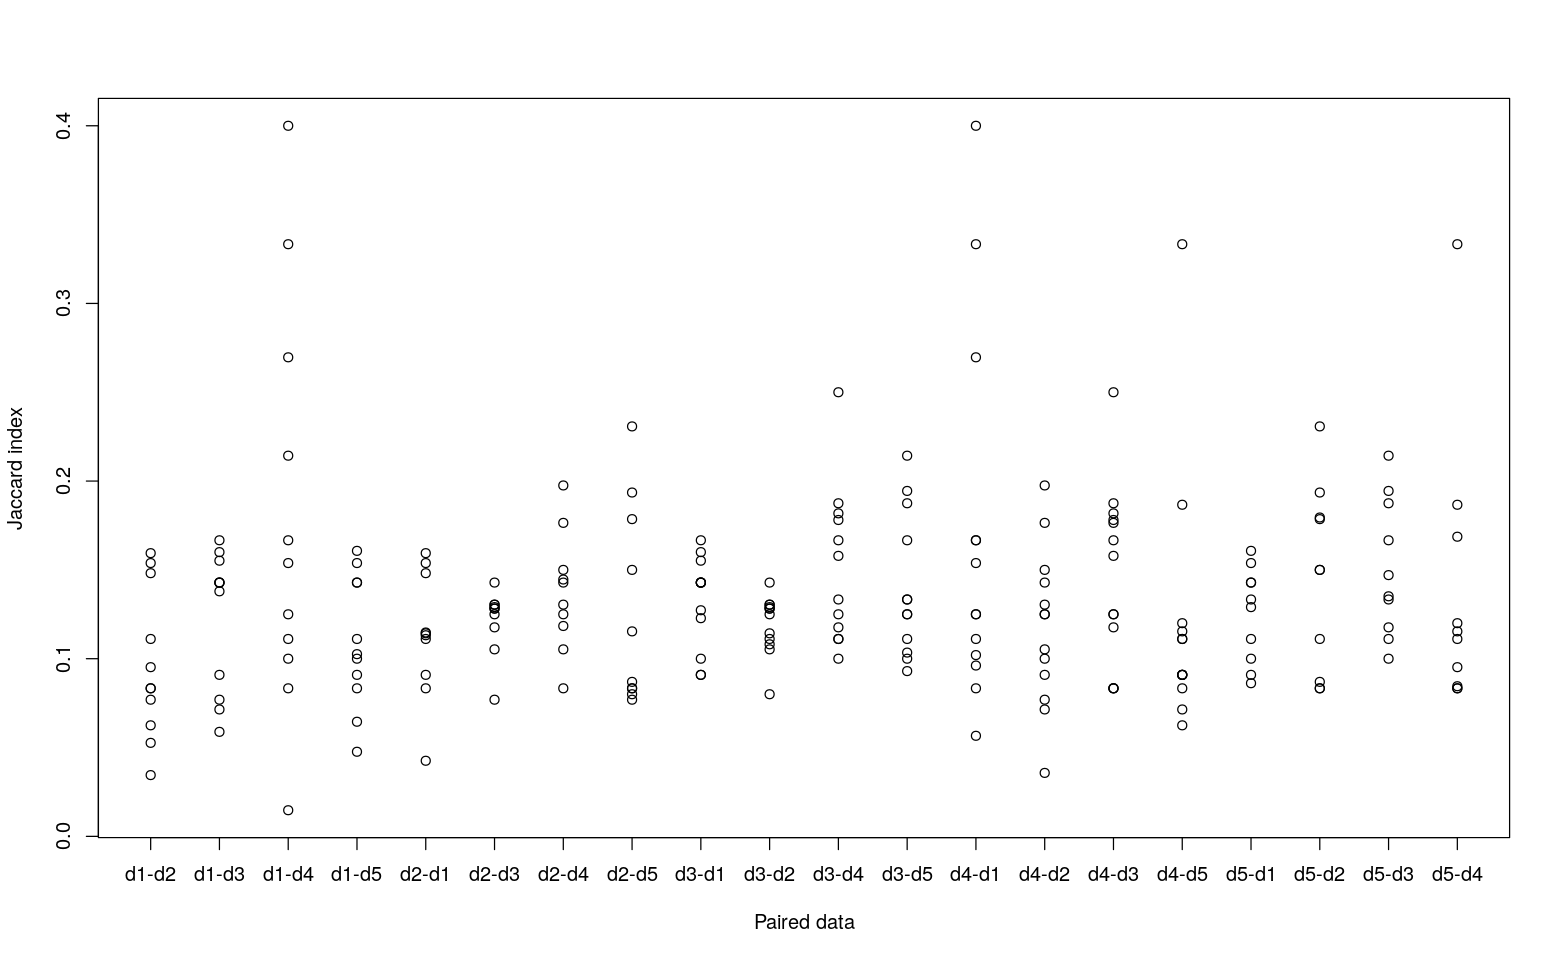
\includegraphics[width=\linewidth]{dd-jaccard}
				\caption{阻害睡眠データペアで各クラスタのJaccard係数を計算した図.}
        \label{fig:dd-jaccard}
    \end{center}
\end{figure}
\begin{figure}[htbp]
    \begin{center}
				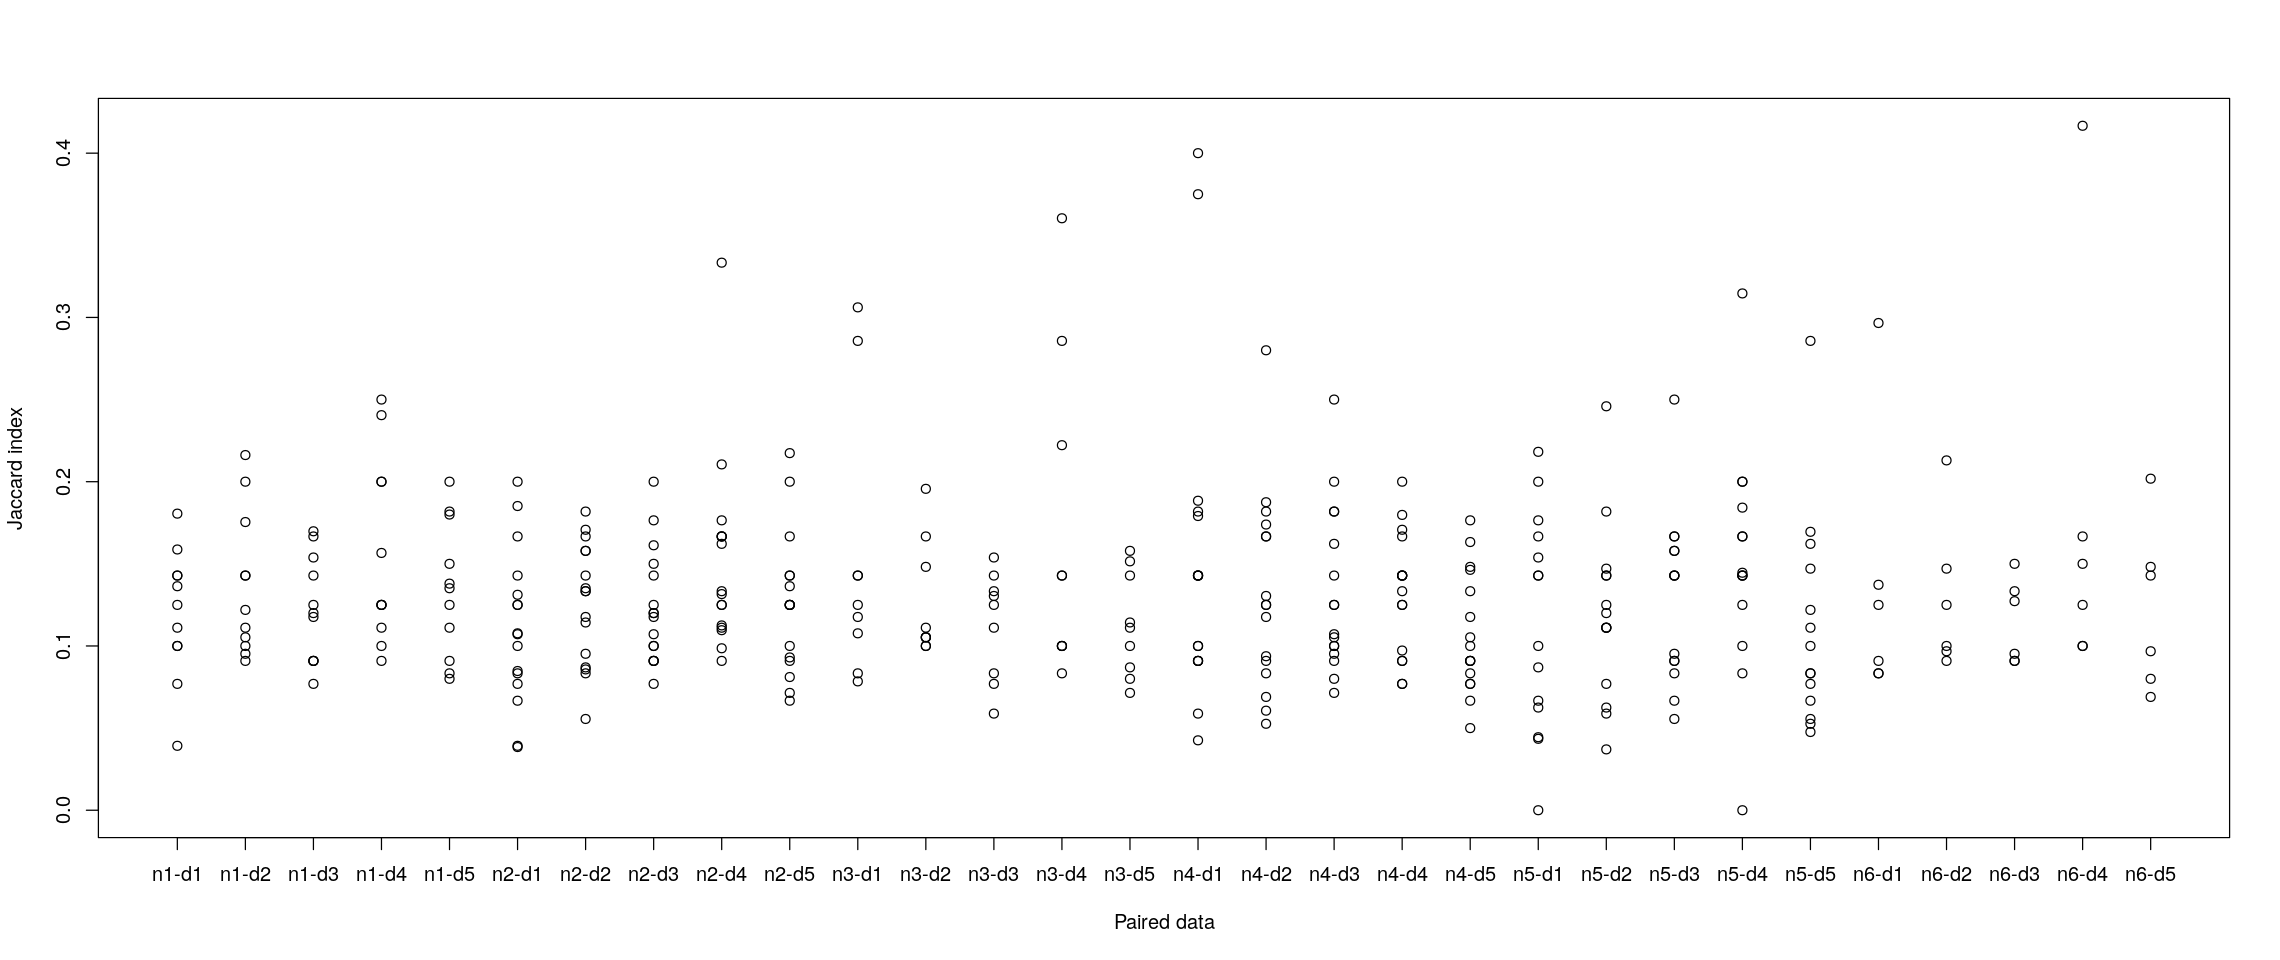
\includegraphics[width=\linewidth]{dn-jaccard}
				\caption{通常睡眠データと阻害睡眠データで各クラスタのJaccard係数を計算した図.}
        \label{fig:dn-jaccard}
    \end{center}
\end{figure}

\subsection{相互相関行列との比較}
前節で提案アプローチによって捉えた睡眠中の大規模クラスタを,相互相関行列から抽出できるかを検証する.
15分間のデータそれぞれについて相互相関行列を計算し,相互相関行列をそのまま用いた場合と$k$近傍法で$k$の数を変化させた場合と$\varepsilon$近傍法で$\varepsilon$を変化させた場合にスペクトラルクラスタリングを行う.
$k$の値は10,20,30,40,50として,閾値$\varepsilon$は相互相関行列の上から20,30,40,50[\%]の値とした.
クラスタ数は前節同様プログラムを用いて自動で決定したが,クラスタ数があまりに大きすぎる場合に目視で判断できるデータに対しては目視で決定した.

相互相関行列をそのまま用いた場合と$k$近傍法を用いた場合に推定されたクラスタのクラスタ内ニューロン数を\Figref{fig:corr-clstnums}に示す.
相互相関行列そのままの場合や$k$が小さい場合はうまくクラスタ数が決められず1つのニューロンのクラスタができている.
また,$k$を大きくした場合でも,睡眠中のデータで大規模クラスタは見受けられない.

$\varepsilon$近傍法を用いた時の推定クラスタ内ニューロン数を\Figref{fig:corre-clstnums}に示す.
閾値が上から30[\%]や40[\%]の時は睡眠中データでの大規模クラスタは見られるが,20[\%]と50[\%]の時には見られない.
閾値によって結果が変化してしまうため,閾値を決める必要のない点で提案アプローチの方が良いと考えられる.

\begin{figure}[htbp]
    \begin{minipage}{0.49\hsize}
			\begin{center}
					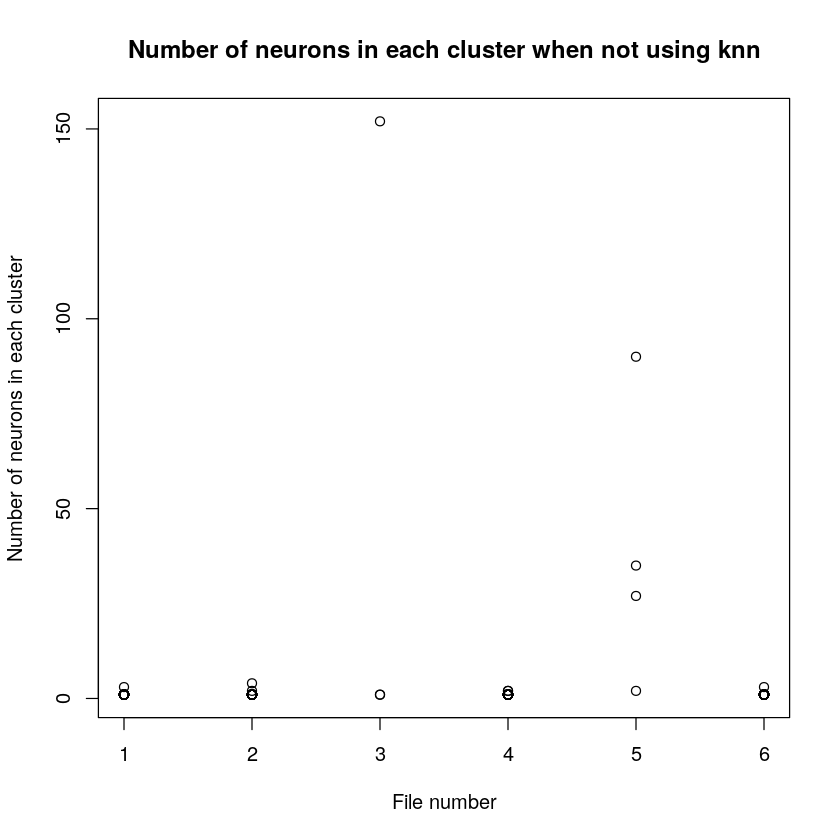
\includegraphics[width=\hsize]{corr-clstnums0}
			\end{center}
		\end{minipage}
    \begin{minipage}{0.49\hsize}
			\begin{center}
					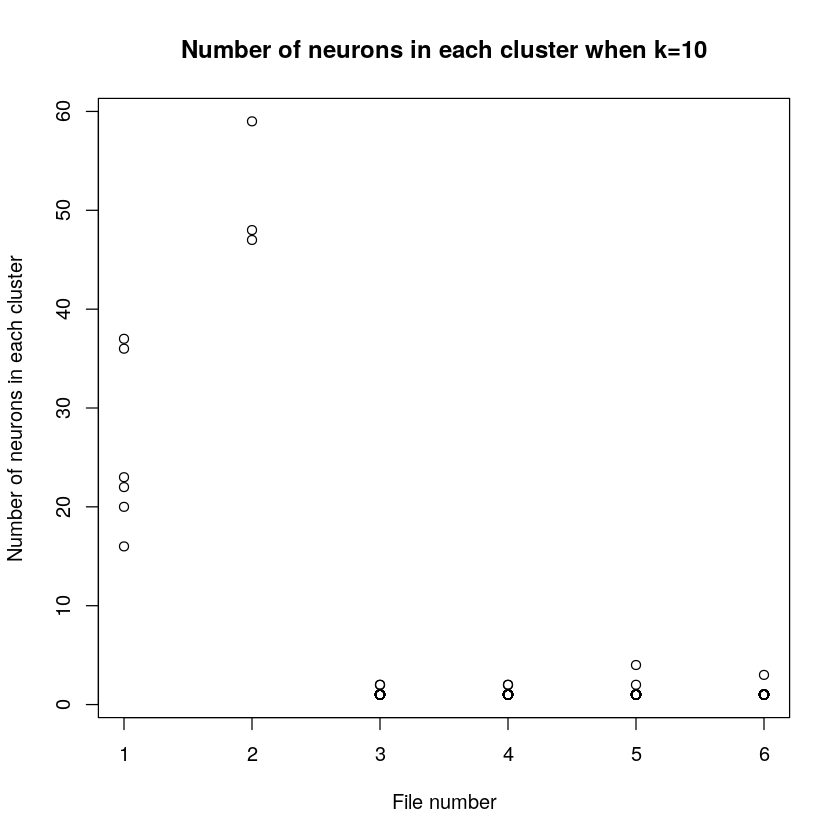
\includegraphics[width=\hsize]{corr-clstnums10}
			\end{center}
		\end{minipage}\\
    \begin{minipage}{0.49\hsize}
			\begin{center}
					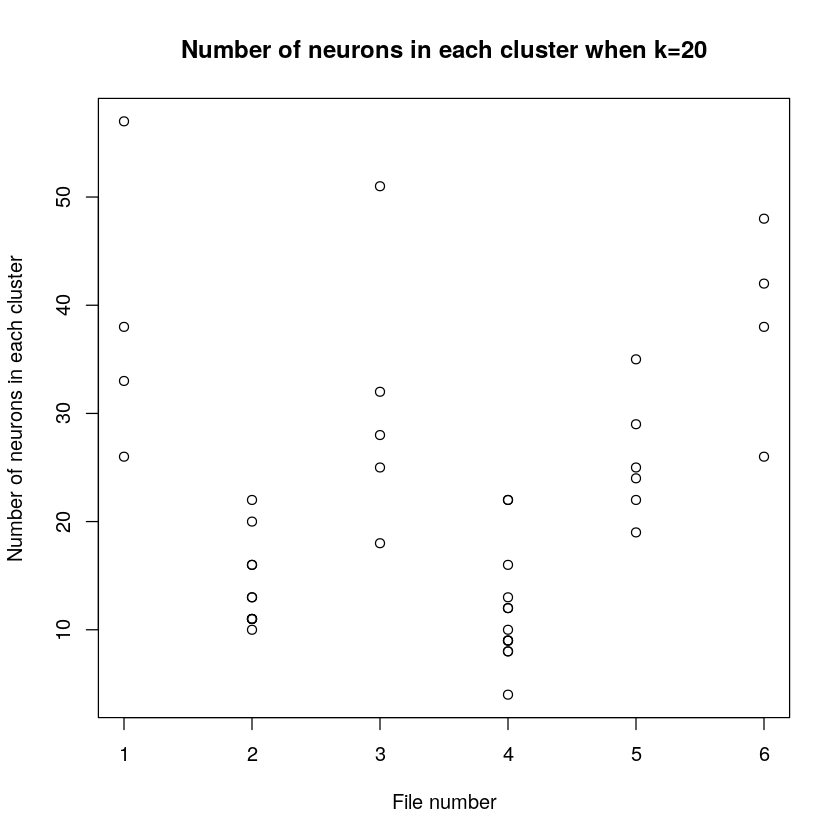
\includegraphics[width=\hsize]{corr-clstnums20}
			\end{center}
		\end{minipage}
    \begin{minipage}{0.49\hsize}
			\begin{center}
					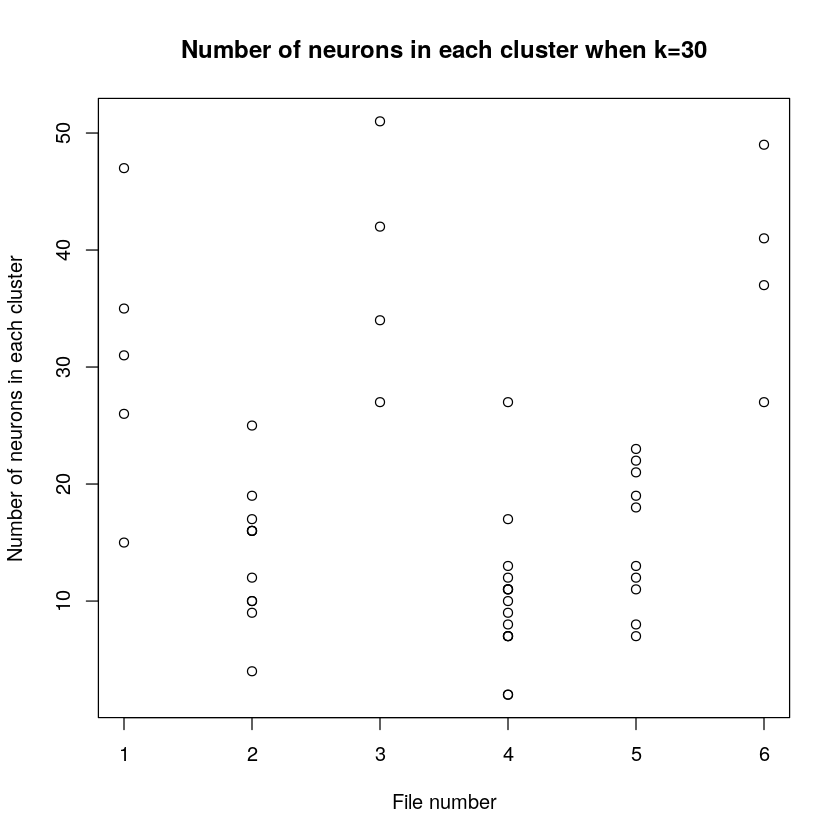
\includegraphics[width=\hsize]{corr-clstnums30}
			\end{center}
		\end{minipage}\\
    \begin{minipage}{0.49\hsize}
			\begin{center}
					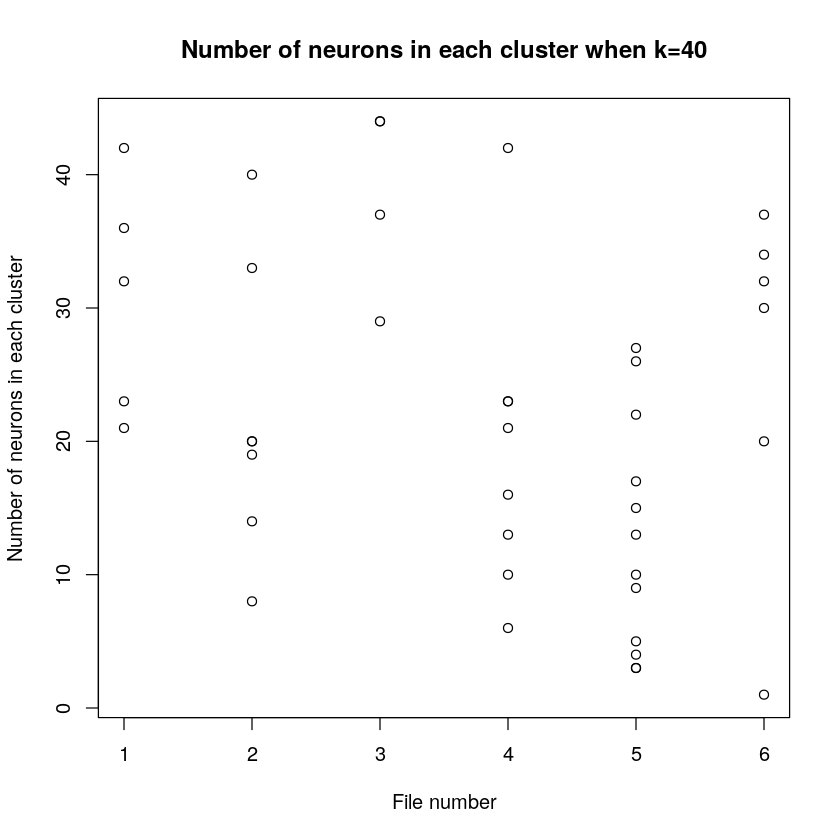
\includegraphics[width=\hsize]{corr-clstnums40}
			\end{center}
		\end{minipage}
    \begin{minipage}{0.49\hsize}
			\begin{center}
					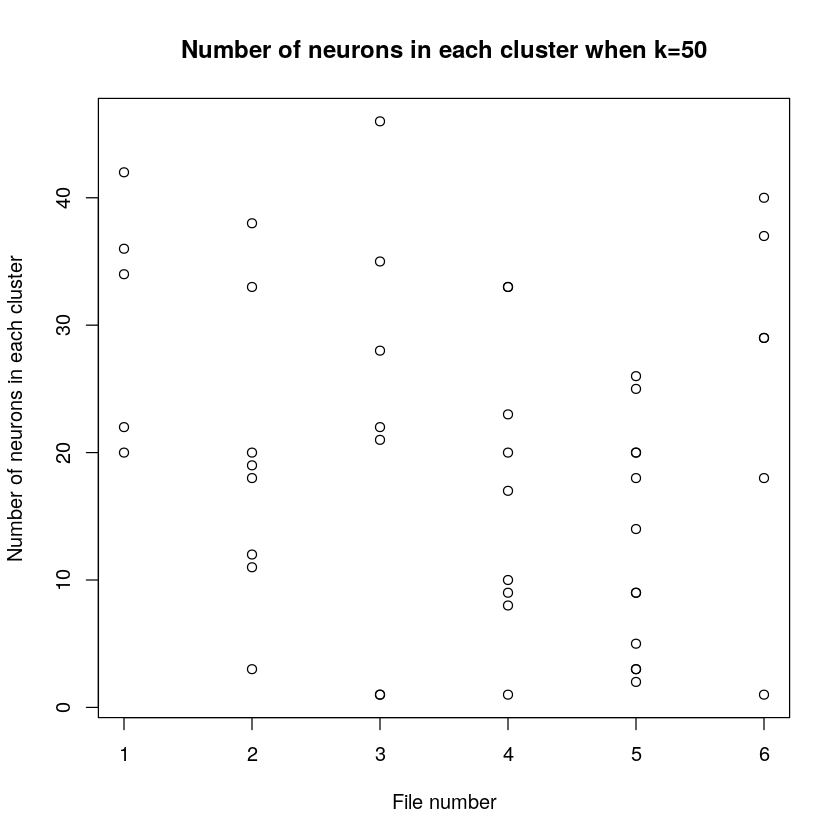
\includegraphics[width=\hsize]{corr-clstnums50}
			\end{center}
		\end{minipage}
		\label{fig:corr-clstnums}
		\caption{$k$近傍法の$k$を変化させた時のクラスタ内ニューロン数.左上は$k$近傍法を用いず相互相関行列のまま用いてスペクトラルクラスタリングを行ったもの.}
\end{figure}
\begin{figure}[htbp]
    \begin{minipage}{0.49\hsize}
			\begin{center}
					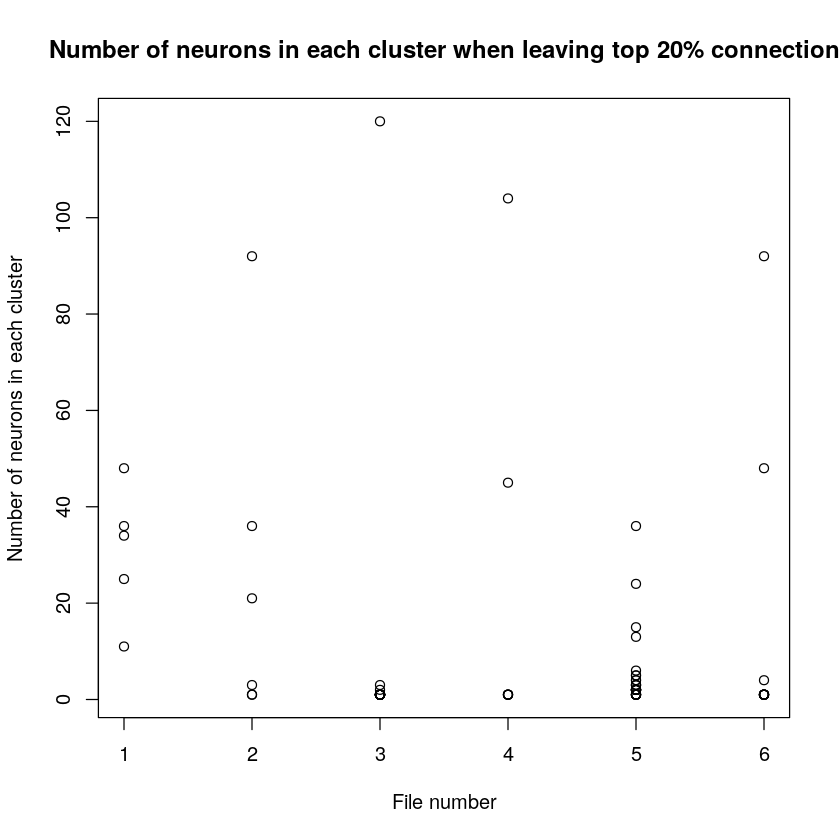
\includegraphics[width=\hsize]{corre-clstnums20}
			\end{center}
		\end{minipage}
    \begin{minipage}{0.49\hsize}
			\begin{center}
					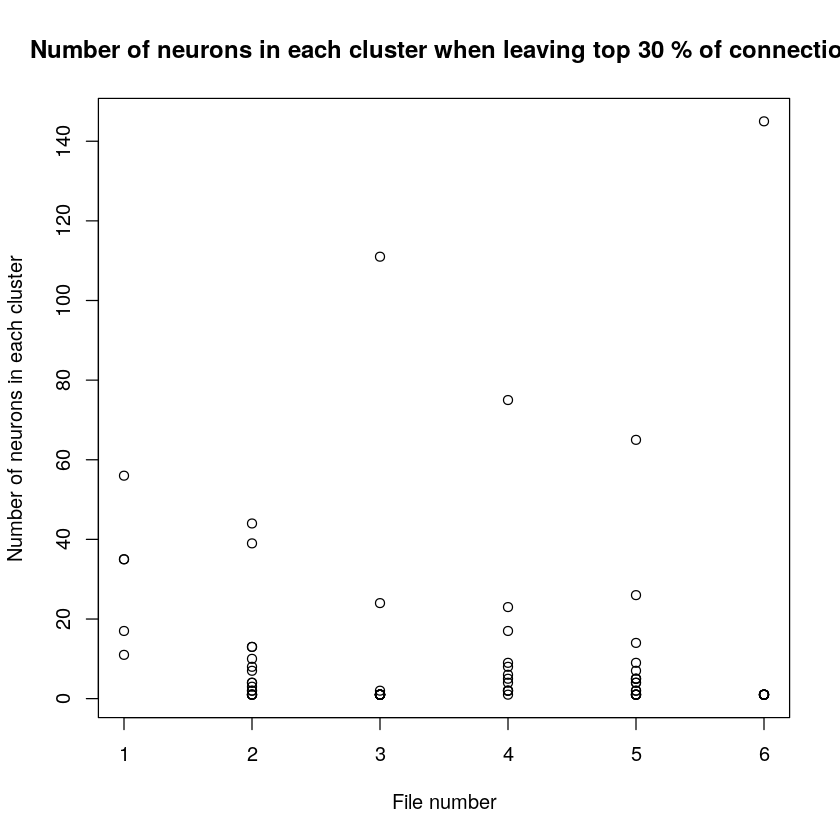
\includegraphics[width=\hsize]{corre-clstnums30}
			\end{center}
		\end{minipage}\\
    \begin{minipage}{0.49\hsize}
			\begin{center}
					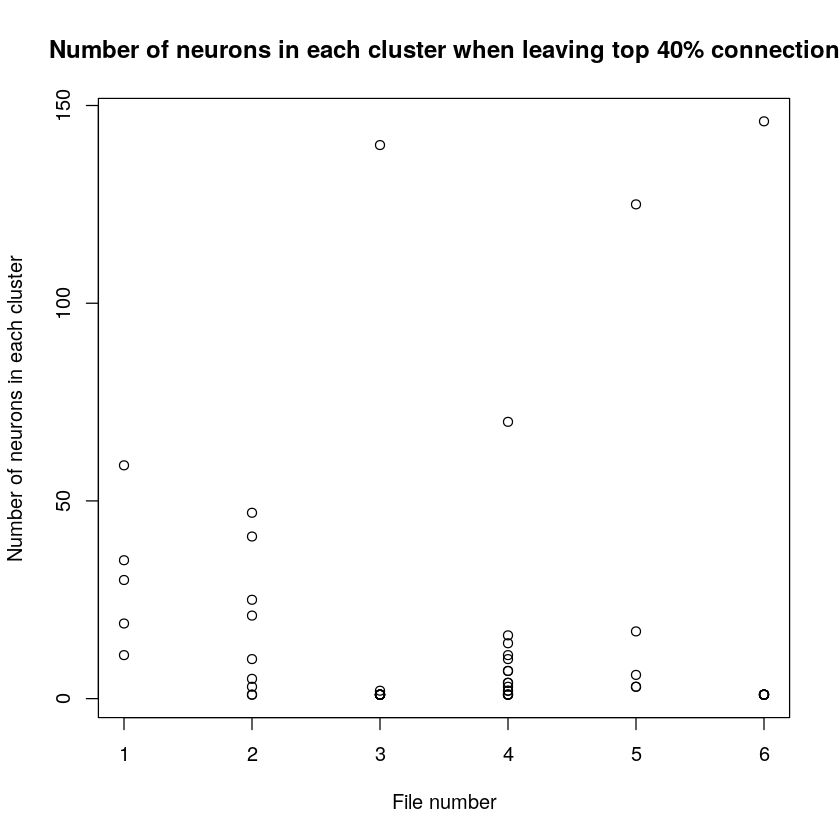
\includegraphics[width=\hsize]{corre-clstnums40}
			\end{center}
		\end{minipage}
    \begin{minipage}{0.49\hsize}
			\begin{center}
					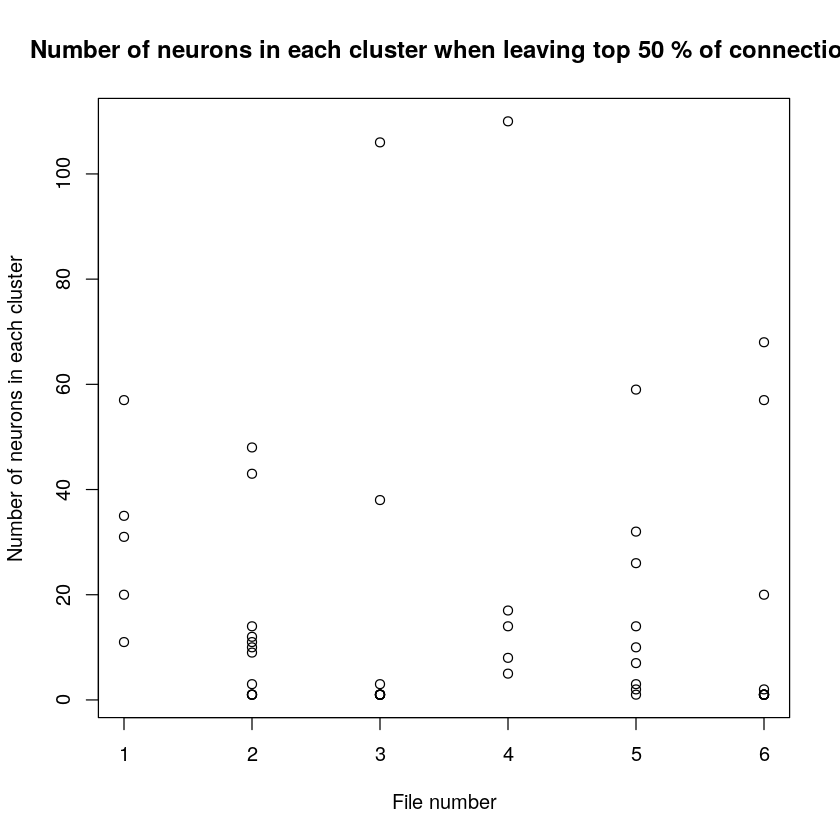
\includegraphics[width=\hsize]{corre-clstnums50}
			\end{center}
		\end{minipage}
		\label{fig:corre-clstnums}
		\caption{$\epsilon$近傍法の$\epsilon$を変化させた時のクラスタ内ニューロン数.$\epsilon$の値は相互相関行列の上から何[\%]までの値とした.}
\end{figure}
